\documentclass[14pt]{extbook}
\usepackage{multicol, enumerate, enumitem, hyperref, color, soul, setspace, parskip, fancyhdr} %General Packages
\usepackage{amssymb, amsthm, amsmath, bbm, latexsym, units, mathtools} %Math Packages
\everymath{\displaystyle} %All math in Display Style
% Packages with additional options
\usepackage[headsep=0.5cm,headheight=12pt, left=1 in,right= 1 in,top= 1 in,bottom= 1 in]{geometry}
\usepackage[usenames,dvipsnames]{xcolor}
\usepackage{dashrule}  % Package to use the command below to create lines between items
\newcommand{\litem}[1]{\item#1\hspace*{-1cm}\rule{\textwidth}{0.4pt}}
\pagestyle{fancy}
\lhead{Progress Quiz 3}
\chead{}
\rhead{Version A}
\lfoot{3148-2249}
\cfoot{}
\rfoot{Spring 2021}
\begin{document}

\begin{enumerate}
\litem{
Construct the lowest-degree polynomial given the zeros below. Then, choose the intervals that contain the coefficients of the polynomial in the form $x^3+bx^2+cx+d$.\[ 5 + 3 i \text{ and } -3 \]\begin{enumerate}[label=\Alph*.]
\item \( b \in [7, 11], c \in [2.8, 4.9], \text{ and } d \in [-111, -99] \)
\item \( b \in [-13, -3], c \in [2.8, 4.9], \text{ and } d \in [92, 105] \)
\item \( b \in [-5, 2], c \in [-5.1, -1], \text{ and } d \in [-19, -11] \)
\item \( b \in [-5, 2], c \in [-1.5, 3.7], \text{ and } d \in [-13, -7] \)
\item \( \text{None of the above.} \)

\end{enumerate} }
\litem{
Construct the lowest-degree polynomial given the zeros below. Then, choose the intervals that contain the coefficients of the polynomial in the form $ax^3+bx^2+cx+d$.\[ \frac{-5}{3}, \frac{7}{2}, \text{ and } \frac{3}{5} \]\begin{enumerate}[label=\Alph*.]
\item \( a \in [30, 34], b \in [-76, -69], c \in [-148, -138], \text{ and } d \in [-107, -100] \)
\item \( a \in [30, 34], b \in [68, 75], c \in [-148, -138], \text{ and } d \in [-107, -100] \)
\item \( a \in [30, 34], b \in [-174, -166], c \in [267, 273], \text{ and } d \in [-107, -100] \)
\item \( a \in [30, 34], b \in [-76, -69], c \in [-148, -138], \text{ and } d \in [104, 107] \)
\item \( a \in [30, 34], b \in [36, 39], c \in [-208, -198], \text{ and } d \in [104, 107] \)

\end{enumerate} }
\litem{
Which of the following equations \textit{could} be of the graph presented below?
\begin{center}
    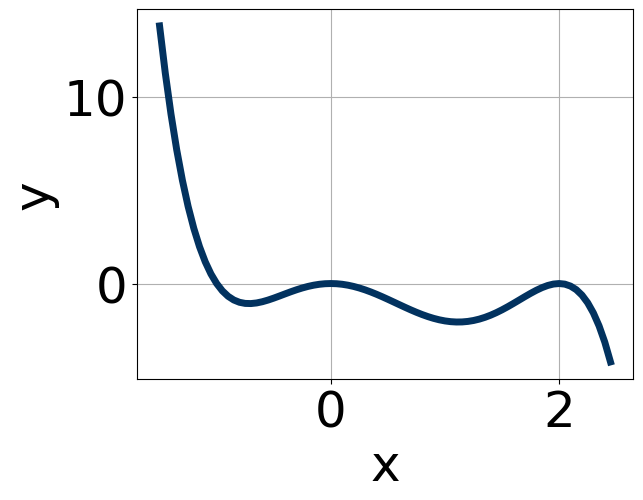
\includegraphics[width=0.5\textwidth]{../Figures/polyGraphToFunctionA.png}
\end{center}
\begin{enumerate}[label=\Alph*.]
\item \( -14x^{6} (x - 2)^{10} (x + 1)^{9} \)
\item \( 6x^{6} (x - 2)^{8} (x + 1)^{11} \)
\item \( 20x^{10} (x - 2)^{6} (x + 1)^{8} \)
\item \( -4x^{10} (x - 2)^{5} (x + 1)^{9} \)
\item \( -8x^{10} (x - 2)^{7} (x + 1)^{8} \)

\end{enumerate} }
\litem{
Describe the end behavior of the polynomial below.\[ f(x) = -9(x + 5)^{3}(x - 5)^{6}(x + 2)^{2}(x - 2)^{4} \]\begin{enumerate}[label=\Alph*.]
\begin{multicols}{2}\item 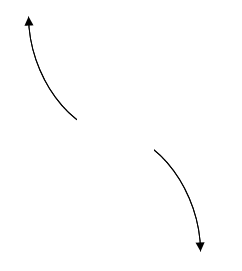
\includegraphics[width = 0.3\textwidth]{../Figures/polyEndBehaviorCopyAA.png}\item 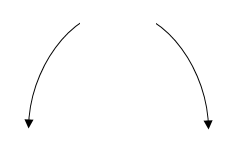
\includegraphics[width = 0.3\textwidth]{../Figures/polyEndBehaviorCopyBA.png}\item 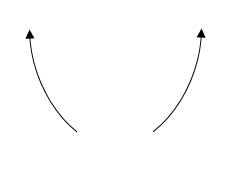
\includegraphics[width = 0.3\textwidth]{../Figures/polyEndBehaviorCopyCA.png}\item 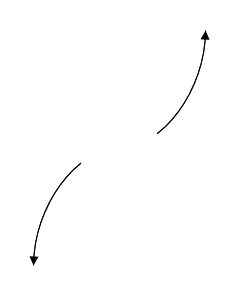
\includegraphics[width = 0.3\textwidth]{../Figures/polyEndBehaviorCopyDA.png}\end{multicols}\item None of the above.
\end{enumerate} }
\litem{
Construct the lowest-degree polynomial given the zeros below. Then, choose the intervals that contain the coefficients of the polynomial in the form $ax^3+bx^2+cx+d$.\[ 1, 5, \text{ and } \frac{-3}{5} \]\begin{enumerate}[label=\Alph*.]
\item \( a \in [4, 15], b \in [32, 36], c \in [41, 45], \text{ and } d \in [10, 17] \)
\item \( a \in [4, 15], b \in [19, 30], c \in [1, 17], \text{ and } d \in [-17, -11] \)
\item \( a \in [4, 15], b \in [-24, -14], c \in [-50, -34], \text{ and } d \in [-17, -11] \)
\item \( a \in [4, 15], b \in [-33, -26], c \in [1, 17], \text{ and } d \in [10, 17] \)
\item \( a \in [4, 15], b \in [-33, -26], c \in [1, 17], \text{ and } d \in [-17, -11] \)

\end{enumerate} }
\litem{
Which of the following equations \textit{could} be of the graph presented below?
\begin{center}
    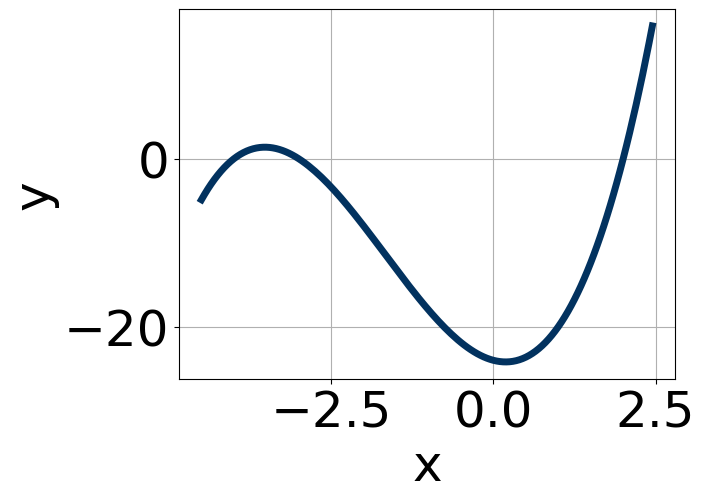
\includegraphics[width=0.5\textwidth]{../Figures/polyGraphToFunctionCopyA.png}
\end{center}
\begin{enumerate}[label=\Alph*.]
\item \( 14(x - 2)^{11} (x - 3)^{5} (x + 4)^{5} \)
\item \( -6(x - 2)^{5} (x - 3)^{9} (x + 4)^{11} \)
\item \( 4(x - 2)^{6} (x - 3)^{5} (x + 4)^{11} \)
\item \( 7(x - 2)^{10} (x - 3)^{10} (x + 4)^{7} \)
\item \( -15(x - 2)^{4} (x - 3)^{9} (x + 4)^{5} \)

\end{enumerate} }
\litem{
Describe the zero behavior of the zero $x = -9$ of the polynomial below.\[ f(x) = 5(x + 4)^{12}(x - 4)^{8}(x - 9)^{9}(x + 9)^{8} \]\begin{enumerate}[label=\Alph*.]
\begin{multicols}{2}\item 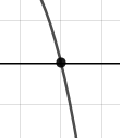
\includegraphics[width = 0.3\textwidth]{../Figures/polyZeroBehaviorAA.png}\item 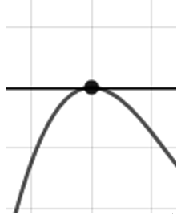
\includegraphics[width = 0.3\textwidth]{../Figures/polyZeroBehaviorBA.png}\item 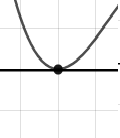
\includegraphics[width = 0.3\textwidth]{../Figures/polyZeroBehaviorCA.png}\item 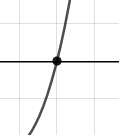
\includegraphics[width = 0.3\textwidth]{../Figures/polyZeroBehaviorDA.png}\end{multicols}\item None of the above.
\end{enumerate} }
\litem{
Construct the lowest-degree polynomial given the zeros below. Then, choose the intervals that contain the coefficients of the polynomial in the form $x^3+bx^2+cx+d$.\[ 4 - 5 i \text{ and } 4 \]\begin{enumerate}[label=\Alph*.]
\item \( b \in [1, 11], c \in [-11, 0], \text{ and } d \in [10, 17] \)
\item \( b \in [3, 13], c \in [71, 75], \text{ and } d \in [163, 167] \)
\item \( b \in [1, 11], c \in [-2, 6], \text{ and } d \in [-27, -17] \)
\item \( b \in [-16, -8], c \in [71, 75], \text{ and } d \in [-165, -163] \)
\item \( \text{None of the above.} \)

\end{enumerate} }
\litem{
Describe the zero behavior of the zero $x = 9$ of the polynomial below.\[ f(x) = 4(x + 9)^{8}(x - 9)^{9}(x + 8)^{9}(x - 8)^{10} \]\begin{enumerate}[label=\Alph*.]
\begin{multicols}{2}\item 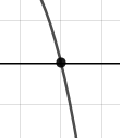
\includegraphics[width = 0.3\textwidth]{../Figures/polyZeroBehaviorCopyAA.png}\item 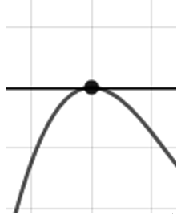
\includegraphics[width = 0.3\textwidth]{../Figures/polyZeroBehaviorCopyBA.png}\item 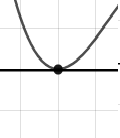
\includegraphics[width = 0.3\textwidth]{../Figures/polyZeroBehaviorCopyCA.png}\item 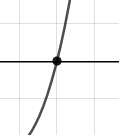
\includegraphics[width = 0.3\textwidth]{../Figures/polyZeroBehaviorCopyDA.png}\end{multicols}\item None of the above.
\end{enumerate} }
\litem{
Describe the end behavior of the polynomial below.\[ f(x) = 2(x - 8)^{4}(x + 8)^{5}(x - 6)^{2}(x + 6)^{3} \]\begin{enumerate}[label=\Alph*.]
\begin{multicols}{2}\item 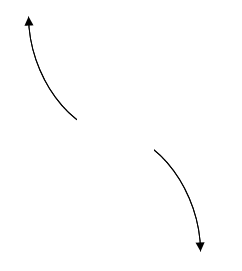
\includegraphics[width = 0.3\textwidth]{../Figures/polyEndBehaviorAA.png}\item 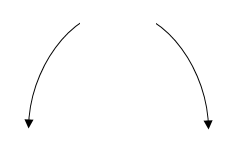
\includegraphics[width = 0.3\textwidth]{../Figures/polyEndBehaviorBA.png}\item 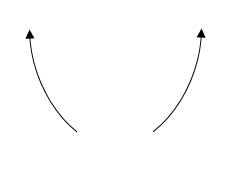
\includegraphics[width = 0.3\textwidth]{../Figures/polyEndBehaviorCA.png}\item 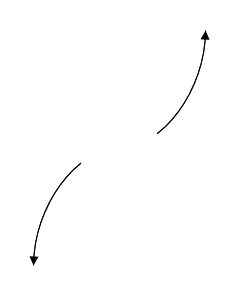
\includegraphics[width = 0.3\textwidth]{../Figures/polyEndBehaviorDA.png}\end{multicols}\item None of the above.
\end{enumerate} }
\end{enumerate}

\end{document}